%start preamble
\documentclass[paper=a4,fontsize=11pt]{scrartcl}%kind of doc, font size, paper size

\usepackage{fontspec}
\defaultfontfeatures{Ligatures=TeX}
%\setsansfont{Liberation Sans}
\usepackage{polyglossia}	
\setdefaultlanguage{german}	
		
\usepackage{amsmath}%get math done
\usepackage{amsthm}%get theorems and proofs done
\usepackage{graphicx}%get pictures & graphics done
\graphicspath{{pictures/}}%folder to stash all kind of pictures etc
\usepackage{amssymb}%symbolics for math
\usepackage{amsfonts}%extra fonts
\usepackage []{natbib}%citation style
\usepackage{caption}%captions under everything
\usepackage{listings}
\usepackage[titletoc]{appendix}
\numberwithin{equation}{section} 
\usepackage[printonlyused,withpage]{acronym}%how to handle acronyms
\usepackage{float}%for garphics and how to let them floating around in the doc
\usepackage{cclicenses}%license!
\usepackage{xcolor}%nicer colors, here used for links
\usepackage{wrapfig}%making graphics floated by text and not done by minipage
\usepackage{dsfont}
\usepackage{stmaryrd}
\usepackage{geometry}
\usepackage{hyperref}
\usepackage{fancyhdr}
\usepackage{menukeys}
\usepackage{csquotes}

\pagestyle{fancy}
\lhead{Netzwerke und verteilte Systeme\\
 Übung\\ Wintersemester 2021/22}
\rhead{FB-4\\Informatik in Kultur und Gesundheit\\ HTW-Berlin}
\lfoot{Virtualisierung mit VirtualBox}
\cfoot{}
\fancyfoot[R]{\thepage}
\renewcommand{\headrulewidth}{0.4pt}
\renewcommand{\footrulewidth}{0.4pt}

\lstdefinestyle{Bash}{
  language=bash,
  showstringspaces=false,
  basicstyle=\small\sffamily,
  numbers=left,
  numberstyle=\tiny,
  numbersep=5pt,
  frame=trlb,
  columns=fullflexible,
  backgroundcolor=\color{gray!20},
  linewidth=0.9\linewidth,
  %xleftmargin=0.5\linewidth
}

%settings colors for links
\hypersetup{
    colorlinks,
    linkcolor={blue!50!black},
    citecolor={blue},
    urlcolor={blue!80!black}
}

\newlength\labelwd
\settowidth\labelwd{\bfseries viii.)}
\usepackage{tasks}
\settasks{counter-format =tsk[a].), label-format=\bfseries, label-offset=3em, label-align=right, label-width
=\labelwd, before-skip =\smallskipamount, after-item-skip=0pt}
\usepackage[inline]{enumitem}
\setlist[enumerate]{% (
labelindent = 0pt, leftmargin=*, itemsep=12pt, label={\textbf{\arabic*.)}}}


%%here begins the actual document%%
\newcommand{\horrule}[1]{\rule{\linewidth}{#1}} % Create horizontal rule command with 1 argument of height

\DeclareMathOperator{\id}{id}

\begin{document}
\begin{center}
\Large{\textbf{Nutzung von Virtualisierung -- VirtualBox}}
\end{center}
\begin{center}\Large{\textbf{Virtualisierungssoftware}}\end{center}\vskip0.25in
Virtualisierungsumgebungen sind Programmpakete, die es ermöglichen auf einem physischen Rechner weitere logische Rechner in Software zu simulieren. In diesen virtuellen Maschinen (VMs) kann ein Betriebssystem, wie auf einem physischen Rechner, mit beliebiger Software (sofern von der Emulation erlaubt) betrieben werden.\\
Eine kurze Auswahl von Virtualisierungsumgebungen:
\begin{itemize}
	\item libvirt \url{https://libvirt.org/} -- Multi-Hypervisor -- Linux
	\item bhyve \url{https://wiki.freebsd.org/bhyve} -- FreeBSD
	\item XEN: \url{http://www.xenproject.org} -- Linux
	\item Oracle VirtualBox: \url{http://www.virtualbox.org} -- Multi-Plattform
	\item Parallels Desktop: \url{http://www.parallels.com} -- OSx
	\item vmWare: \url{http://www.vmware.com} -- Multi-Plattform
\end{itemize}

\begin{center}
\Large{\textbf{virtualBox im Labor}}
\end{center}
Im Labor sind alle PCs mit zwei physischen Netzwerkkarten ausgestattet. Damit ist es möglich die Rechner an zwei unterschiedliche Netzwerke anzuschließen. Ein Anschluss verbindet den Rechner mit allen anderen Rechnern der HTW-Berlin, dem Internet und sorgt dafür, dass sie sich z.B. beim Betriebssystem anmelden können. Diese Verbindung wird auf allen Rechnern mit dem grauem Netzwerkkabel hergestellt.
\begin{figure}[H]
	\centering
	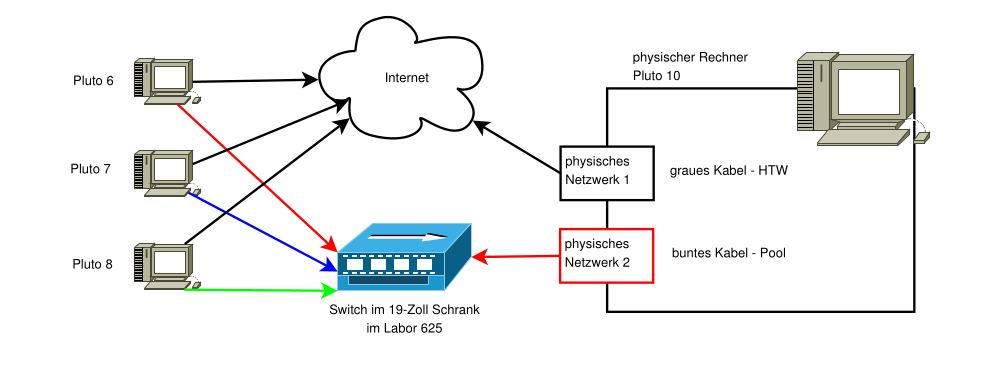
\includegraphics[scale=0.4]{wh_c_625}
\end{figure}
Das zweite Kabel ist bunt und spannt ein weiteres Netz auf, welches nur innerhalb des Labors verfügbar ist. Dieses Netzwerk hat ebenfalls eine Anbindung an das restliche Hochschulnetz, ist jedoch durch den Laborrouter abgeschirmt. Für unsere Übungen werden wir (solange nichts anderes gesagt ist) in diesem Netzwerk arbeiten -- hier können wir beliebige Netzwerkeinstellungen vornehmen oder Routing-Protokolle und Netzwerkdienste starten ohne das es zu Problemen im Netzwerk der Hochschule kommt.
\begin{center}
\Large{\textbf{Virtuelle Maschinen}}
\end{center}
Eine Virtuelle Maschine besteht bei allen Systemen (virtualBox, VMWare, ...) aus einer Konfigurationsdatei, in der die simulierte Hardware festgelegt wird und einer oder mehrerer großer Dateien, die als Massenspeicher der VM dienen. Zum Verschieben einer virtuellen Maschine auf einen anderen Rechner müssen sie einfach das Verzeichnis mit diesen Dateien kopieren.\\

Wenn nach dem Start der VM ein Dialogfenster mit der Frage kommt, ob Sie diese VM verschoben oder kopiert haben, sollten Sie im Labor \enquote{kopiert} antworten. Grund hierfür sind die von der VM genutzten MAC-Adressen -- bei verschobenen VMs bleiben die MAC-Adressen gleich, bei  \enquote{kopierten} generiert virtualBox automatisch neue MAC-Adressen. Somit ist sichergestellt, dass es keine doppelten MAC-Adressen im Pool gibt.\\

Sollte es beim Import einer VM (VirtualBox Manager Program -- Menü: Machine -- Hinzufügen) eine Fehlermeldung geben, dass die Konfigurationsdatei nicht gültig sei, so öffnen Sie diese bitte in einem Texteditor (die *.vbox Datei im Verzeichnis) und prüfen sie die XML-Syntax. Es kam beim Kopieren und automatischen Anpassen der Datei manchmal vor, das ein schließende spitze Klammer am Ende nicht richtig gesetzt wurde.

\begin{center}
\Large{\textbf{Importieren der VM}}
\end{center}
\paragraph{Für das Labor} liegt das Stamm-Image unter \path{/vm/nw_lab} bereit. Diese VM ist nur lesend verfügbar (Read-Only), sodass von ihnen keine Änderungen vorgenommen werden können.\\
\paragraph{Für zu Hause:} Unter folgender URI können Sie das Image herunterladen: \url{https://cloud.htw-berlin.de/s/Gt6XSfrAjqa5PcP}, das Passwort finden sie im Moodle-Kurs, I) Basics.\\
Um die VM zu Hause nutzen zu können, müssen sie eine Virtualisierungsumgebung installiert haben. Die einfachste Variante ist virtualBox. Hier finden sei eine Anleitung, wie virtualBox installiert wird: \url{https://www.virtualbox.org/manual/ch02.html}.\\
\textbf{Beachten sie, dass sie die Virtualisierung ihrer CPU einschalten müssen!} Wie das geht: \url{https://2nwiki.2n.cz/pages/viewpage.action?pageId=75202968}, Im Regelfall ist die Virtualisierung auf modernen CPUs bereits eingeschaltet.\\
Anschließend können sie die VM importieren. Im Menü \emph{Datei/File} gibt es den Eintrag \emph{Importieren (Import Appliance)}, worauf sich eine Dialogbox öffnet in der Sie den Import vornehmen können. \textbf{Im Labor} müssen sie für das zu importierende System \path{/vm/nw_lab/networks.ova} angeben. \textbf{Zu Hause} müssen sie den Download-Pfad des Image angeben. Unter Windows wahrscheinlich \path{Dokumente\Downloads}, bei OSx und Linux zumeist \path{~/Downloads}.\\
Anschließend müssen sie nur noch angeben, wo die VM abzulegen ist und dass die MAC-Adressen neu generiert werden. Beispielhaft ist dies in Abb. \ref{import_vm} zu sehen.
\begin{figure}[H]
	\centering
	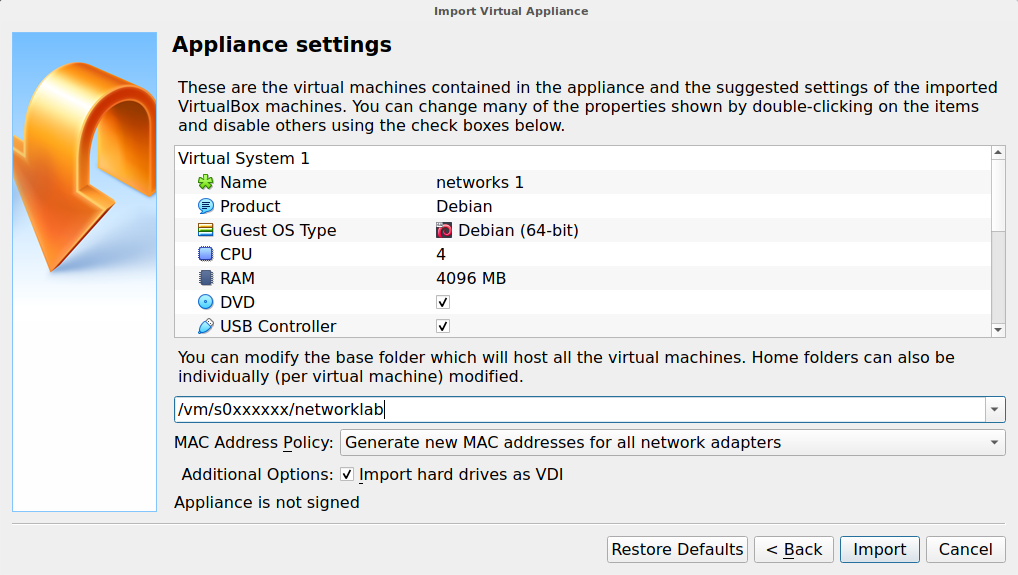
\includegraphics[scale=0.3]{vm_import}
	\caption{Import der VM, zu sehen ist die Konfiguration der VM, mit Pfadangabe und Generierung der MAC-Adressen.}
	\label{import_vm}
\end{figure} 


\begin{center}
\Large{\textbf{Netzwerkeinstellungen der VMs}}
\end{center}
In virtualBox legen sie in den Netzwerkeinstellungen jeder VM fest, wie die realen physischen Netzwerkadapter auf die logischen (also \enquote{simulierten}) Adapter abgebildet werden. Das Host-Betriebssystem muss zwingend wissen, wie und auf welche Ressource das Gast-Betriebssystem (Guest) zugreifen darf. Darüber hinaus wird festgelegt, wie Pakete an diese Adapter weiterzuleiten sind. Diese Einstellungen könne auch zu Laufzeit des Gast-Systems geändert werden -- ein Neustart der VM ist dazu nicht notwendig.
\begin{figure}[H]
	\centering
	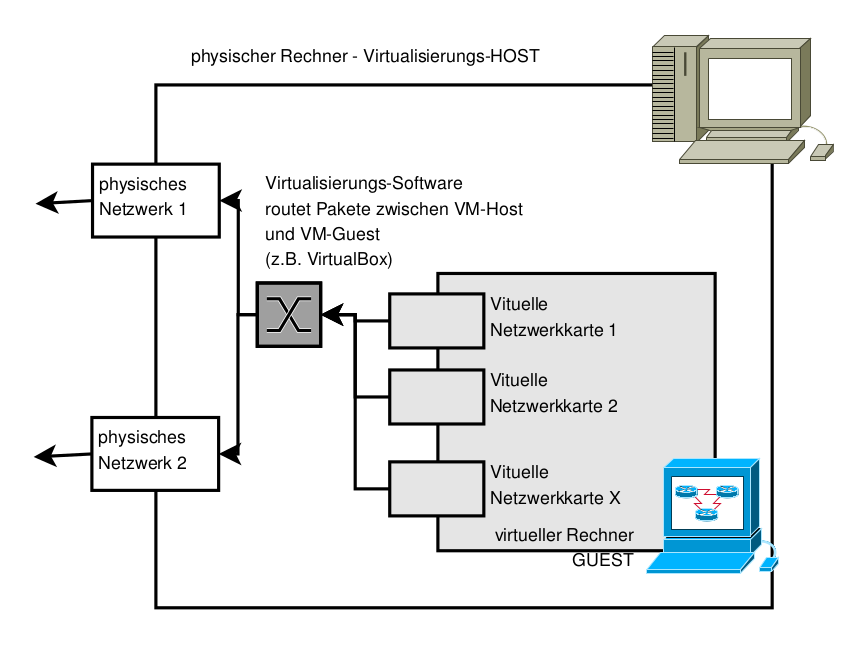
\includegraphics[scale=0.4]{vbox1}
	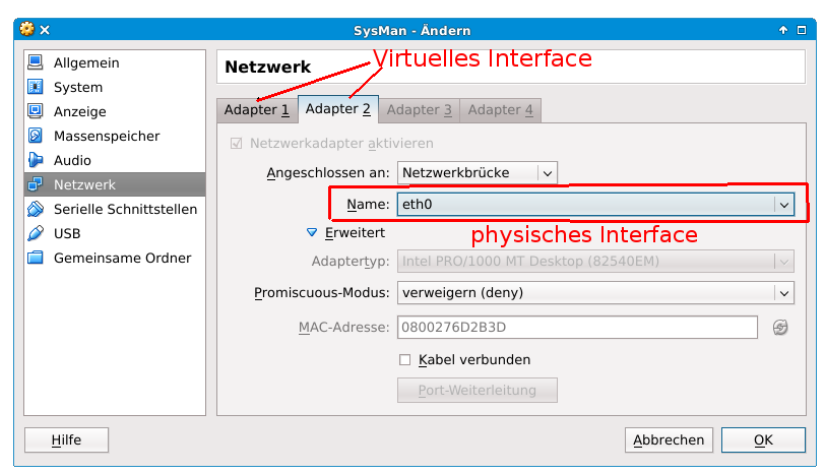
\includegraphics[scale=0.4]{vbox2}
\end{figure}
Im laufenden Betrieb der VM können sie im Fenstermodus unten links mittels des Icons mit den zwei kleinen Monitoren nachschauen, wie die Netzwerkkarten aktuell konfiguriert sind. Dazu warten Sie mit der Maus entweder ein paar Sekunden über dem Icon bis ein kleines Infofenster erscheint (Abbildung \ref{vbox3}) oder, wenn sie mit der rechten Maustaste auf dieses Icon klicken, erhalten sie einen Dialog, mit dem sie die Einstellungen im laufenden Betrieb umstellen können (s. Abb. \ref{vbox4}).
\begin{figure}[H]
\centering
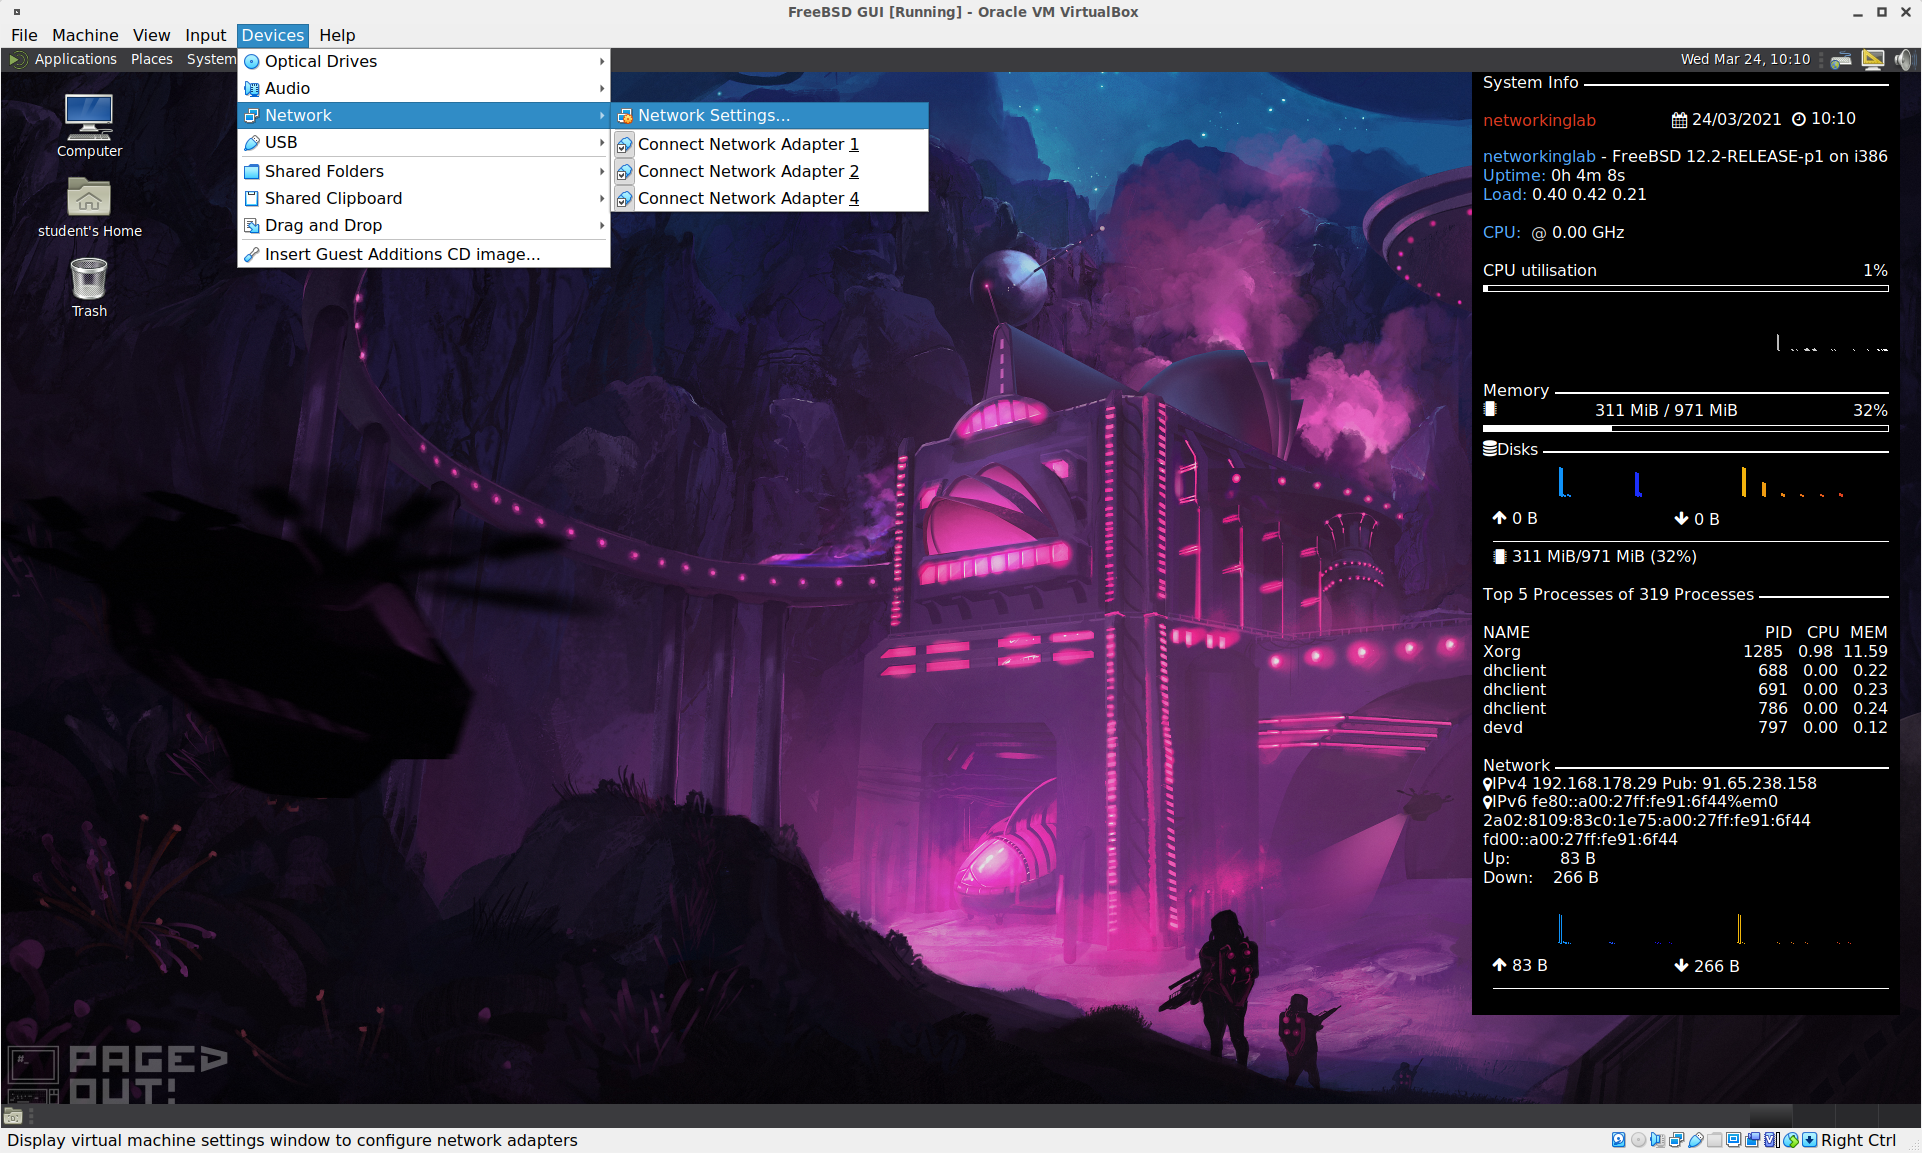
\includegraphics[scale=0.2]{vbox11}
\caption{Zugriff auf Netzwerkeinstellungen via Menüleiste}
\label{vbox3}
\end{figure}
\begin{figure}[H]
\centering
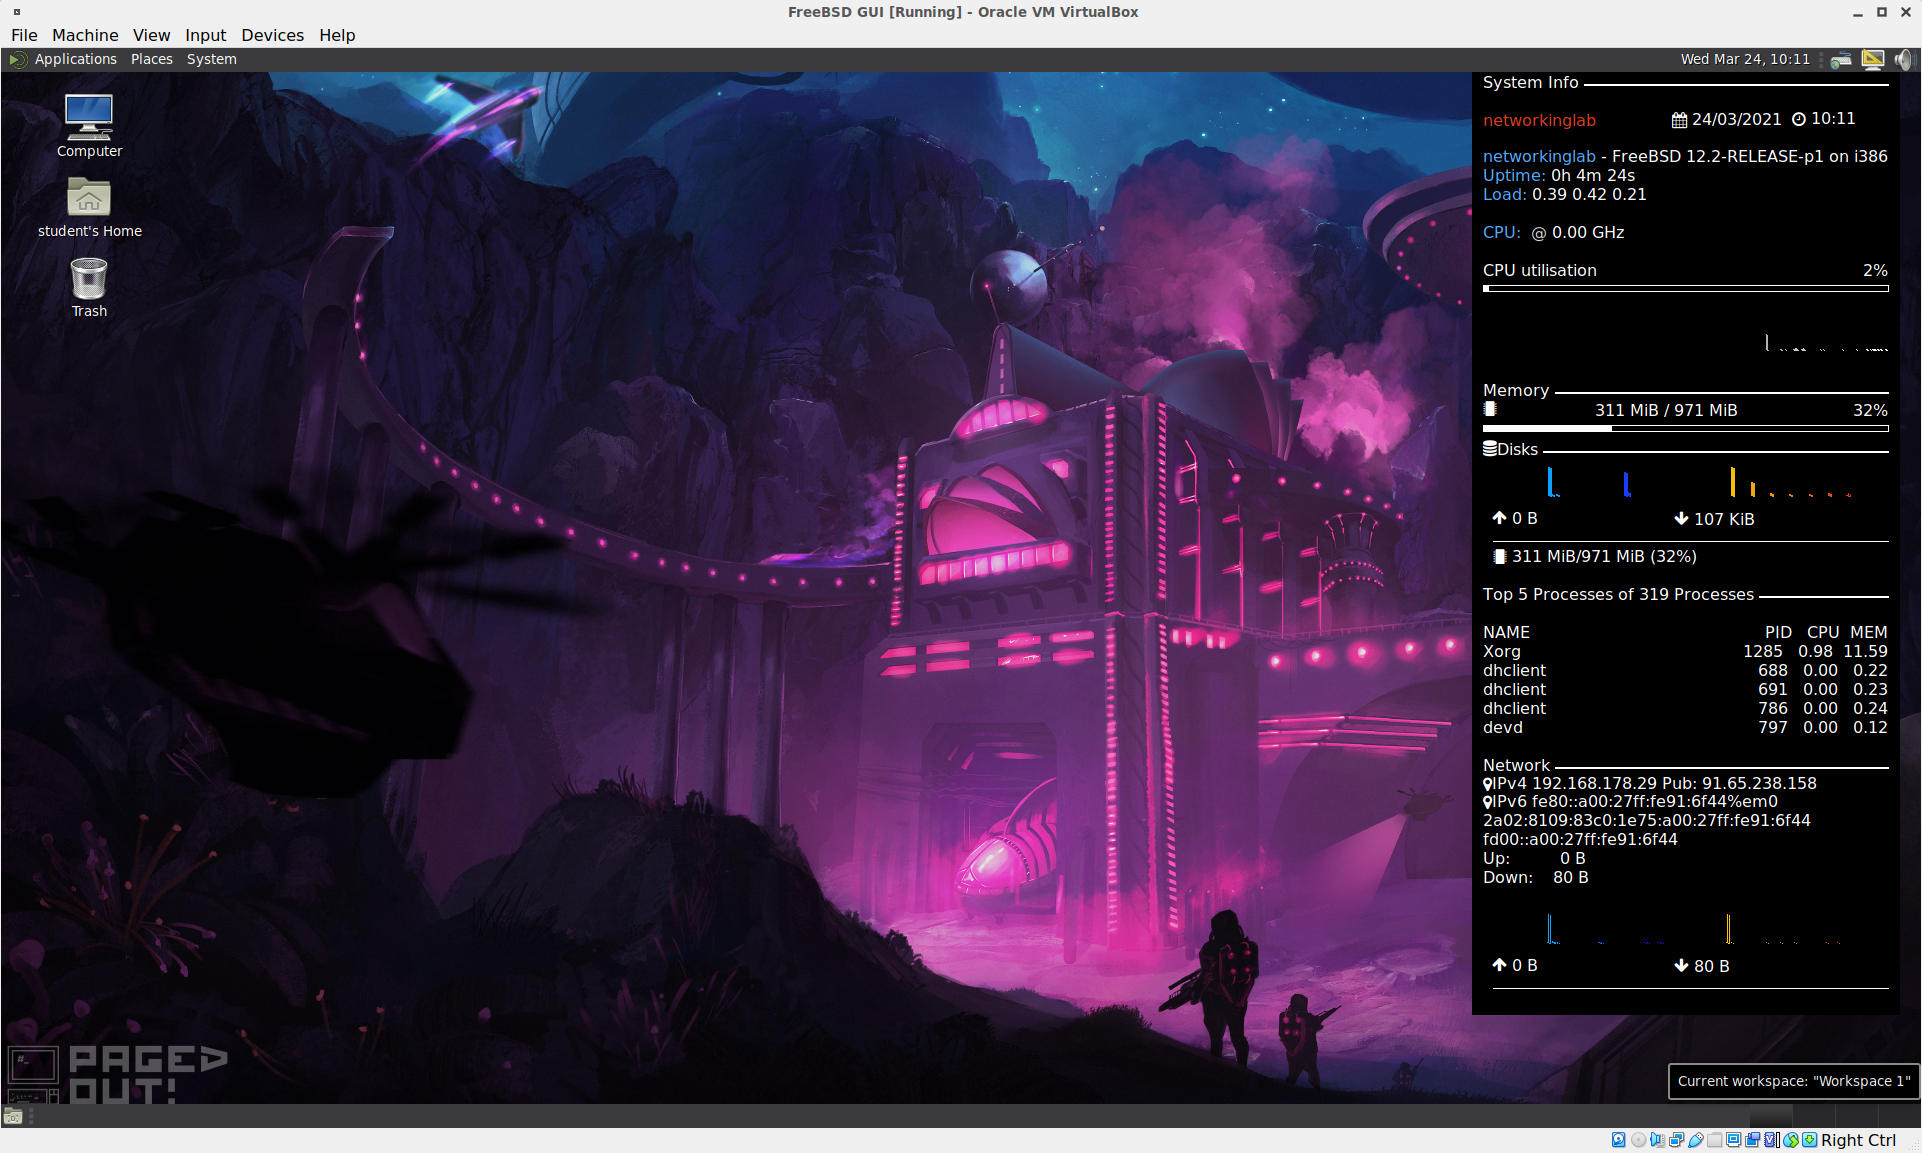
\includegraphics[scale=0.2]{vbox12}
\caption{Zugriff auf Netzwerkeinstellungen via Icons am unteren Rand}
\label{vbox4}
\end{figure}
Bei den Netzwerkkarten können sie mehrere verschiedene Modi einstellen -- für sie interessant sind aber nur drei: Bridge, Host-Only-Adapter und NAT. Die anderen Formen können sie bei Bedarf in der Dokumentation von virtualBox nachlesen (\url{https://www.virtualbox.org/manual/ch06.html}).
\begin{center}
\Large{\textbf{Netzwerkmodus: NAT}}
\end{center}
Im Modus NAT werden alle Netzwerkpakete bevor sie von virtualBox von der VM zum physischen Rechner weitergeleitet werden, umgeschrieben. Damit ist es möglich, dass nach außen die gleiche IP-Adresse Ihres Routers genutzt werden kann. Dies wird in den meisten Fällen unter IPv4 ohnehin getan. NAT kapselt also das Netzwerk in dem Ihre VM arbeitet von dem physischen (NAT) Netzwerk ab.
\begin{figure}[H]
\centering
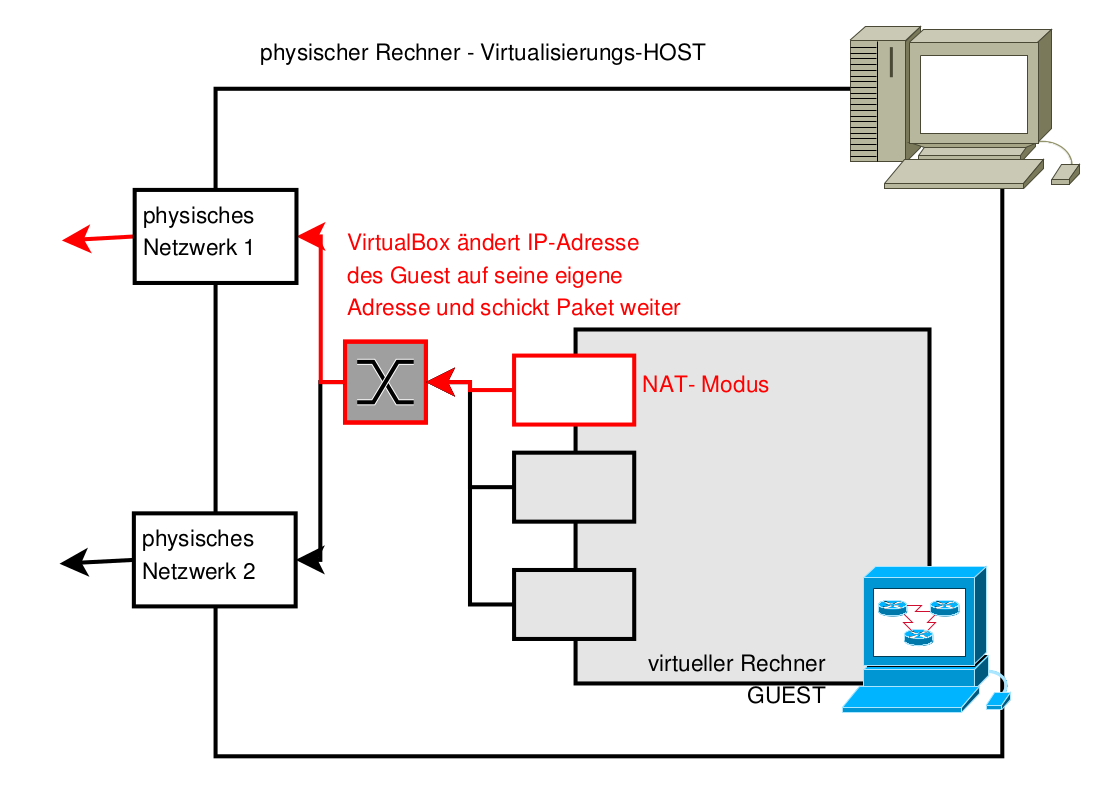
\includegraphics[scale=0.35]{vbox5}
\caption{Virtualisierte Netzwerkkarte im NAT-Modus}
\end{figure}
\begin{center}
\Large{\textbf{Netzwerkmodus: Bridge}}
\end{center}
Im Modus Bridge werden alle von der VM erzeugten Pakete sofort ohne eine Änderung durch virtualBox an die physische Netzwerkkarte weitergereicht und über das Kabel versandt. Dabei muss in den Netzwerkeinstellungen von virtualBox festgelegt werden, auf welche der Netzwerkkarten des physischen Rechners die Pakete weitergeleitet werden -- somit werden Pakete nur an diese eine Netzwerkkarte gesandt. Das genutzte Interface legen sie in den Einstellungen für jedes virtuelle Interface getrennt fest. Zur Laufzeit können sie die Zuordnung auch nachträglich noch ändern. In diesem Modus sieht es für andere Rechner so aus, als ob zwei vollkommen eigenständige Rechner im Netzwerk aktiv sind. Zum einen der physische Host (Rechner) und zum anderen die VM (Guest/Gast). Damit können sich auch alle VMs untereinander direkt per Netzwerk erreichen.
\begin{figure}[H]
\centering
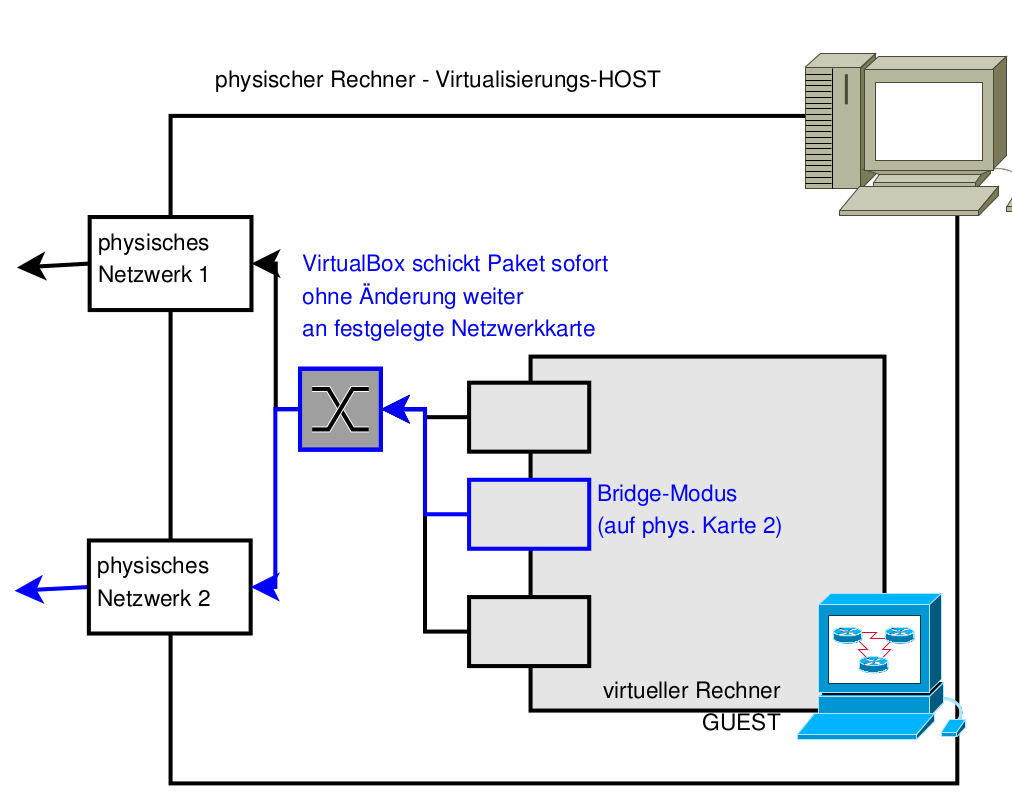
\includegraphics[scale=0.35]{vbox6}
\caption{Virtualisierte Netzwerkkarte im Bridge-Modus}
\end{figure}

\begin{center}
\Large{\textbf{Login \& Admin}}
\end{center}
Wenn die VM korrekt importiert wurde, sollte diese ohne weitere Schwierigkeiten hochfahren. Sie können sich als Nutzer \emph{student} mit dem Passwort \emph{student} anmelden. Der Wechsel des Passworts ist sinnvoll, mit folgenden Befehl können Sie das Standardpasswort ändern. Öffnen sie ein Terminal (via Str+Alt+t).
\begin{lstlisting}[style=Bash, language=Bash]
passwd
\end{lstlisting}
Anschließend werden Sie aufgefordert das alte Passwort anzugeben und anschließend ein neues zu vergeben. Wundern Sie sich nicht, wenn beim Eintippen nichts auf dem Bildschirm zu sehen ist, dies ist ein Sicherheitsfeature.\\
Das Standardpasswort für \emph{root} ist \emph{root}. Der Root-Nutzer ist in Unix-Systemen der Administrator, dieser hat die höchsten Privilegien und darf im System grundsätzlich alles. Sie sollten also aufpassen, was sie machen. Viele Befehle nehmen Kommandos ohne weitere Fragen entgegen und führen diese aus.\\
Im Normalfall sollte der Student-Account ausreichend sein, da dieser der Gruppe \emph{wheel} und \emph{sudo} angehört. Somit kann der Student-Nutzer alle notwendigen Befehle ausführen, die root-Rechte brauchen. Wenn ihnen das System sagt, dass sie nicht ausreichend Rechte zum Ausführen eines Befehls haben, nutzen sie das Präfix \emph{sudo}. Bspw.\\
\begin{lstlisting}[style=Bash, language=Bash]
sudo paris-traceroute 9.9.9.9
\end{lstlisting}
Wenn sie update durchführen wollen, müssen sie wie folgt vorgehen:
\begin{lstlisting}[style=Bash, language=Bash]
sudo pkg update
sudo pkg upgrade -y
\end{lstlisting}
Der erste Befehlt sorgt dafür, dass der Paketkatalog der installierten Software abgeglichen und aktualisiert wird. Der zweite Befehl führt das eigentliche Update durch. 
\end{document}